\documentclass[12pt]{article}

\usepackage{amsmath}
\usepackage{graphicx}
\usepackage{hyperref}
\usepackage{cite}
\usepackage[margin=1.2in]{geometry}

\providecommand{\eqn}[1]{eqn.~(\ref{eqn:#1})}
\providecommand{\tab}[1]{Table~\ref{tab:#1}}
\providecommand{\fig}[1]{Figure~\ref{fig:#1}}

\providecommand{\vecsymbol}[1]{\ensuremath{\boldsymbol{#1}}}
%\providecommand{\pv}{\vecsymbol{p}}
%\providecommand{\deltav}{\vecsymbol{\delta}}

\title{Weather Assumptions for\\
DESI Survey Planning and Forecasts\\
\vspace{5mm}{\large\bf DESI-doc-3087-v1}}
\author{David Kirkby, Kyle Dawson}

\begin{document}
\maketitle

\section{Introduction}

This note briefly summarizes the expected weather-related observing conditions at the Mayall telescope during the five-year DESI survey.  In particular, we cover the expected fraction of nights where the dome remains closed due to weather and the expected distributions of atmospheric seeing and transparency on dome-open nights.  We describe the historical data used as the basis for our assumptions, and algorithms implemented to randomly sample expected weather conditions.

A jupyter notebook to create the plots in this note is provided in the {\tt desimodel} package
under {\tt doc/nb/}.  The LaTeX source for this note is maintained in the same package under {\tt doc/tex/desi3087/}.

\section{Historical Data}

We use metadata collected by the MzLS legacy survey\cite{desi-2947} used to provide imaging data for DESI targeting.  The data was recorded over 233 nights spanning 2015-12-14 to 2017-06-16 and provides timestamps, delivered image quality, and transparency measurements obtained in the z-band.

{\em KD: Provide more details on the MzLS survey conditions and how transparency is defined?}

\subsection{Dome Open Fraction}

The assumed fraction of time that the dome remains closed during each calendar month is summarized in \tab{dome} below. {\em KD: Describe the original source of these numbers and fill in the MzLS stats.}

\begin{table}[htb]
\begin{center}
\begin{tabular}{lcccc}
    Month & Model & Scheduled & Closed & Ratio \\
    \hline
    Jan & 35.24 \\
    Feb & 44.14 \\
    Mar & 27.68 \\
    Apr & 26.73 \\
    May & 14.22 \\
    Jun & 15.78 \\
    Jul & 55.92 \\
    Aug & 48.75 \\
    Sep & 29.45 \\
    Oct & 24.44 \\
    Nov & 24.86 \\
    Dec & 34.74 \\
    \hline
\end{tabular}
\caption{Summary of dome-closed statistics for each calendar month.  The Model column gives the assumed dome-closed fraction in the simulation model.  The remaining columns give the number of scheduled MzLS nights, closed scheduled nights, and their ratio, for comparison.}
\label{tab:dome}
\end{center}
\end{table}

\subsection{Seeing}

We convert the delivered image quality (DIQ) values, reported as full-width half-maximum (FWHM), to atmospheric seeing FWHM values $S$ by subtracting $\sigma = 0.219$ arcsec (RMS) in quadrature to account for the Mosaic instrumental PSF:
$$
s = c \sqrt{(\text{DIQ} / c)^2 - \sigma^2} \quad , \quad c = 2 \sqrt{2\log 2} \; .
$$
We fit the shape of resulting seeing distribution to the parameterization used in~\cite{2014PASP..126..296D},
$$
P(s) = A \left[ 1 + \left(\frac{s-B}{C}\right)^2 \right]^{-D} x^E \;,
$$
obtaining (the parameter $A$ has no influence on the shape of the distribution)
$$
B = 0.0751 \quad,\quad C = 0.443 \quad,\quad D = 23.0 \quad,\quad E = 38.1 \; .
$$
\fig{seeing-fit} shows the resulting fit.

\begin{figure}[htb]
\begin{center}
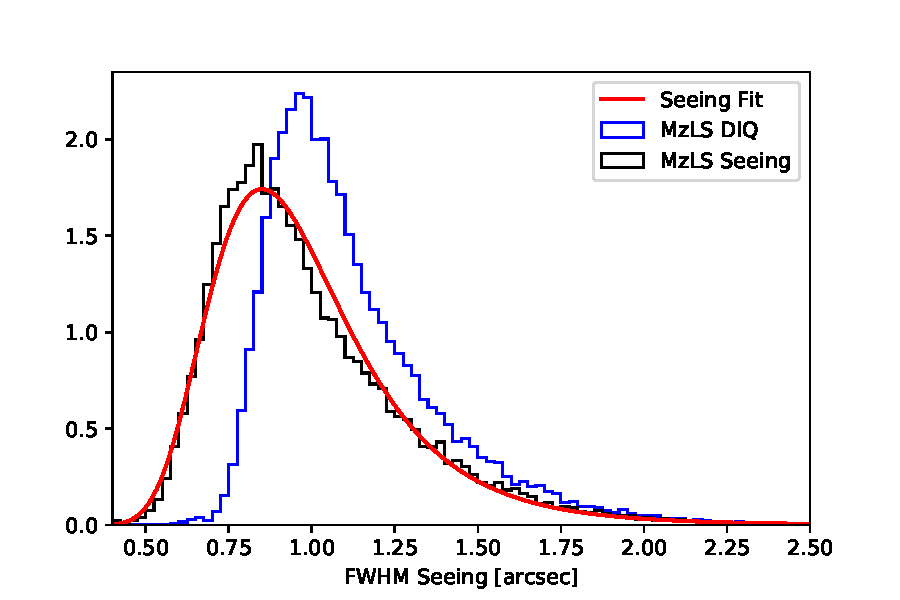
\includegraphics[width=5in]{seeing-fit}
\caption{Distribution of MzLS delivered image quality (DIQ) FWHM values, the corresponding atmospheric seeing FWHM distribution, and a fit to the seeing distribution.}
\label{fig:seeing-fit}
\end{center}
\end{figure}

Atmospheric seeing is expected to improve at redder wavelengths, so the MzLS z-band seeing needs to be adjusted to a wavelength that is more representative of DESI observations.  We define a reference wavelength of 6355\AA, centered in the r-band, for the purposes of survey simulations. Kolmogorov turbulence theory predicts a $\lambda^{-1/5}$ scaling, but the data presented in~\cite{2014PASP..126..296D} is better fit by a much milder $\lambda^{-1/15}$ dependence. Instead of attempting an explicit wavelength correction, we scale the z-band seeing in order to obtain a specified median seeing value, after clipping at $s < 2.5$ arcsec before scaling. In principle, the relationship between the scale factor and the resulring median can be non-linear, but we find that a linear approximation works well (see \fig{seeing-scale}).

\begin{figure}[htb]
\begin{center}
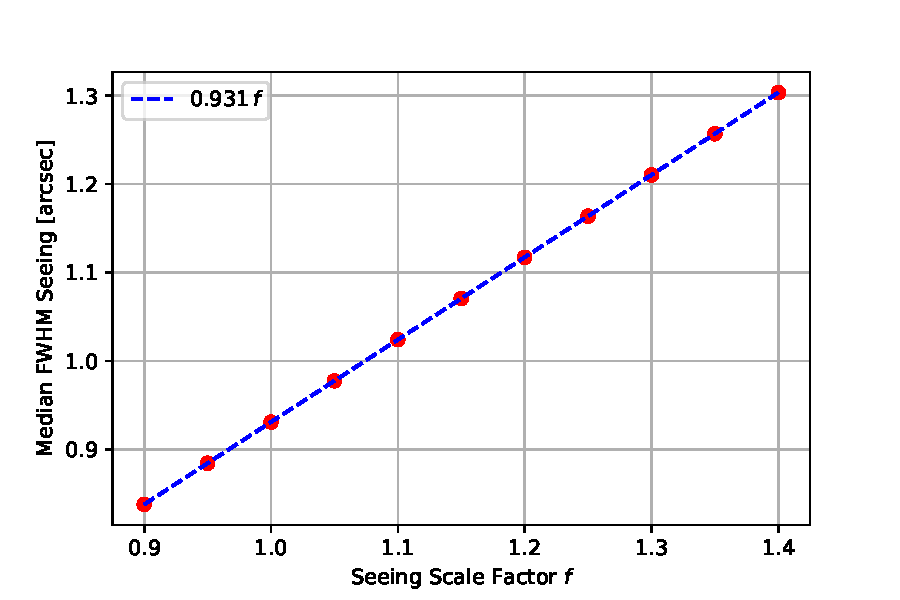
\includegraphics[width=5in]{seeing-scale}
\caption{Median FWHM seeing calculating after applying different scale factors to the MzLS z-band seeing distribution.}
\label{fig:seeing-scale}
\end{center}
\end{figure}

\fig{seeing-pdf} compares seeing distribution scaled to different median values with the original simulation model based on Mosaic data obtained with the ``r SDSS k1018'' filter, as reported in~\cite{2014PASP..126..296D}, which has a median (mean) of 1.156 (1.281) arcsec (truncating at $s < 3$ arcsec).  The nominal 1.1 arcsec median seeing is achieved with a scale factor of $1.18$ (and therefore clipped at $2.95$ arcsec), and a corresponding mean of $1.17$ arcsec.

\begin{figure}[htb]
\begin{center}
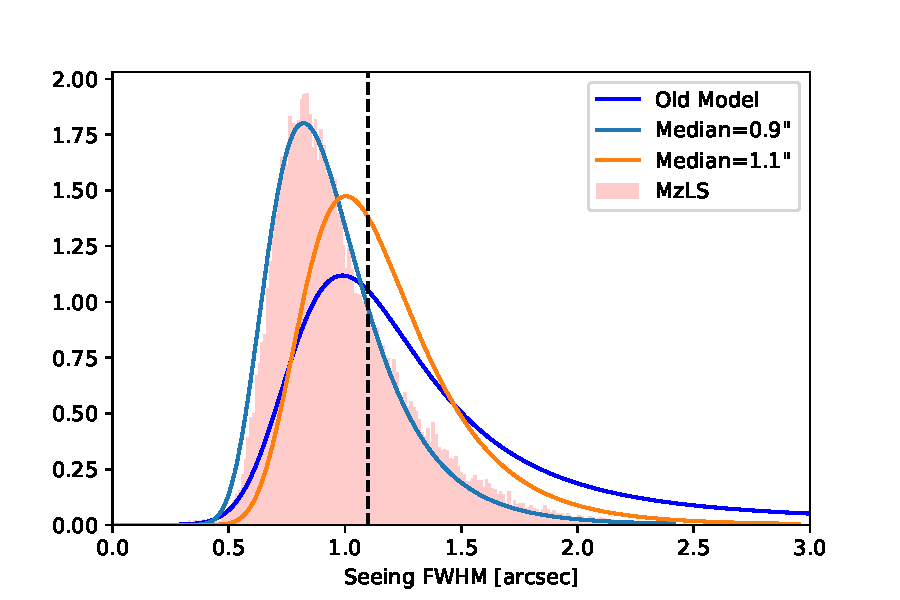
\includegraphics[width=5in]{seeing-pdf}
\caption{Median FWHM seeing calculating after applying different scale factors to the MzLS z-band seeing distribution.}
\label{fig:seeing-pdf}
\end{center}
\end{figure}

\subsection{Transparency}

The raw MzLS transparency values show linear trends that are presumably due to dust accumulation on the primary mirror, as shown in \fig{transp-trend}. We assume that the mirror will be monitored and cleaned frequently enough during DESI observations that we always observe under "just cleaned" conditions. We therefore apply a linear correction to the raw MzLS transparency values, separately in the two periods indicated with colored points in \fig{transp-trend}.  The resulting corrected distributions are compatible for both periods, so we combine them in the following.

\begin{figure}[htb]
\begin{center}
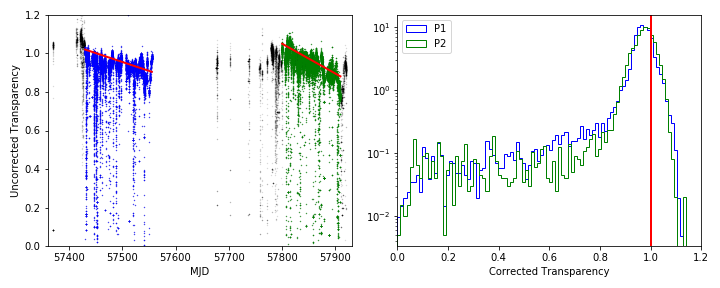
\includegraphics[width=\linewidth]{transp-trend}
\caption{Raw MzLS transparency values over time (left) and the distribution of corrected values (right) obtained during the two periods indicated with colored points.}
\label{fig:transp-trend}
\end{center}
\end{figure}

The corrected transparencies have a tail extending above the limiting value of one for true transparency, which we attribute to Gaussian measurement errors with an RMS of $0.035$, which also shift the peak corrected transparency slightly below one.  We model the corrected transparency distribution as the convolution of a true transparency PDF convolved with a Gaussian. Our true PDF is modeled as a sum of three power laws and truncated to values between zero and one. \fig{transp-model} compares our model with the distribution of corrected transparencies and the original simulation model (a log-normal distribution with mean $0.111$ and RMS $0.333$ truncated between zero and one).  The deconvolved model has a mean of $0.94$ which is only slightly different from the old model's mean of $0.93$, even if their distributions are quite different.

\begin{figure}[htb]
\begin{center}
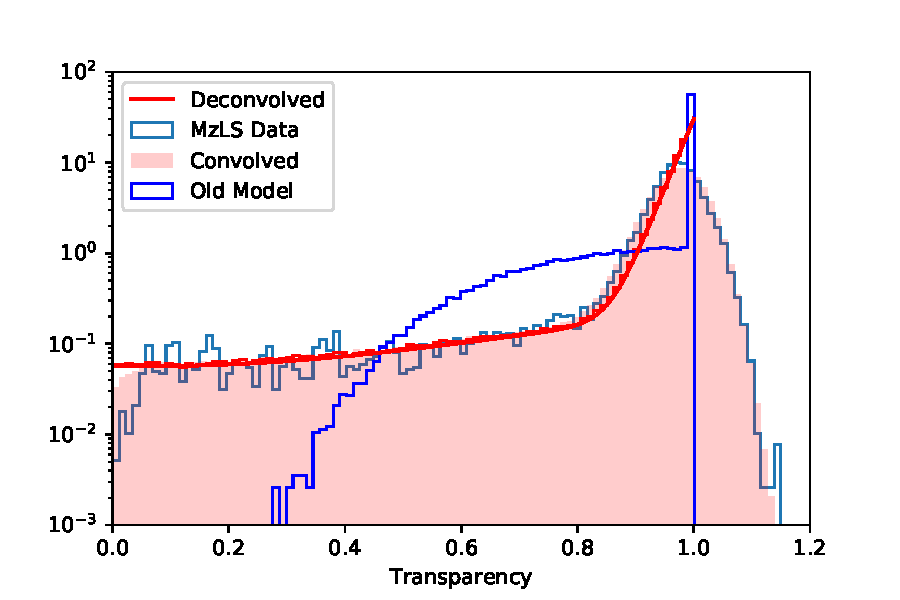
\includegraphics[width=5in]{transp-model}
\caption{Raw MzLS transparency values over time (left) and the distribution of corrected values (right) obtained during the two periods labeled P1 and P2 and indicated with different colored points.}
\label{fig:transp-model}
\end{center}
\end{figure}

\subsection{Time Series Simulation}

In order to simulate conditions during the DESI survey, we need to model their correlated temporal structure and not just their 1D probability density.  Our approach is to estimate the power spectrum of MzLS observations and then generate random realizations of this power covering the 5-year DESI survey.  One complication is that power spectrum is implicitly a Gaussian model of correlated variations, but the distributions of both seeing and transparency are distinctly non-Gaussian.  We deal with this issue using (rank preserving and invertible) ``whitening'' transforms that monotonically maps the target variable (seeing or transparency) to new variable distributed according to a unit Gaussian.

In more detail, we perform the following steps:
\begin{itemize}
    \item Whiten the input values.
    \item Estimate the power spectral density of whitened values (using a Lomb-Scargle periodogram since samples are not equally spaced in time).
    \item Fit the resulting noisy power spectral density (PSD) to a smooth piece-wise power-law function.
    \item Generate random realizations of the PSD fit, constrainted to have zero mean and unit variance.
    \item Apply the inverse whitening transform to the generated values, to recover the 1D probability density of the input values.
\end{itemize}
\fig{power} shows the estimated PSDs and their smooth fits. Note that these are "chi-by-eye" fits, tuned by hand to give realistic simulated time series.  \fig{seeing-sim} and \fig{transp-sim} compares MzLS observations with simulated time series of atmospheric seeing and transparency.

\begin{figure}[htb]
\begin{center}
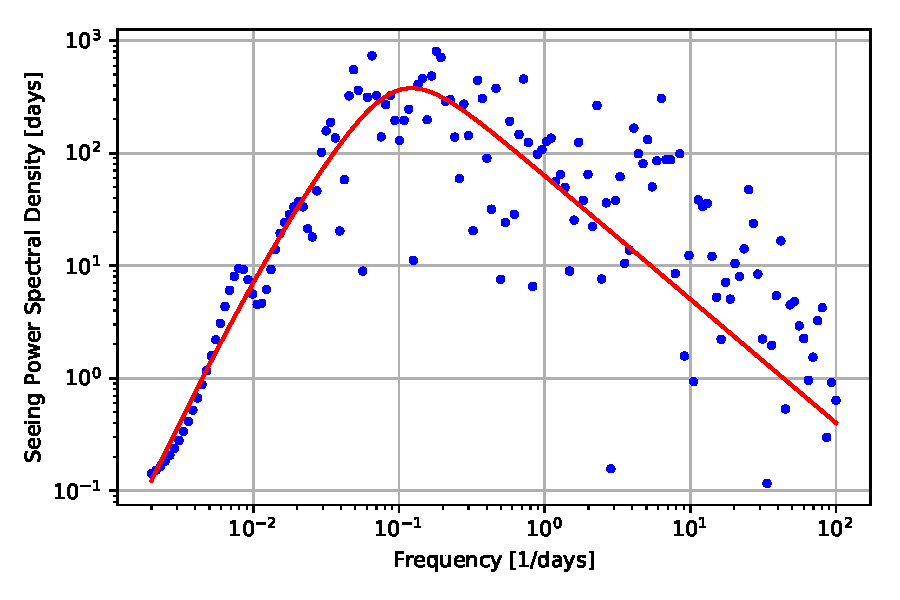
\includegraphics[width=0.48\linewidth]{seeing-psd}
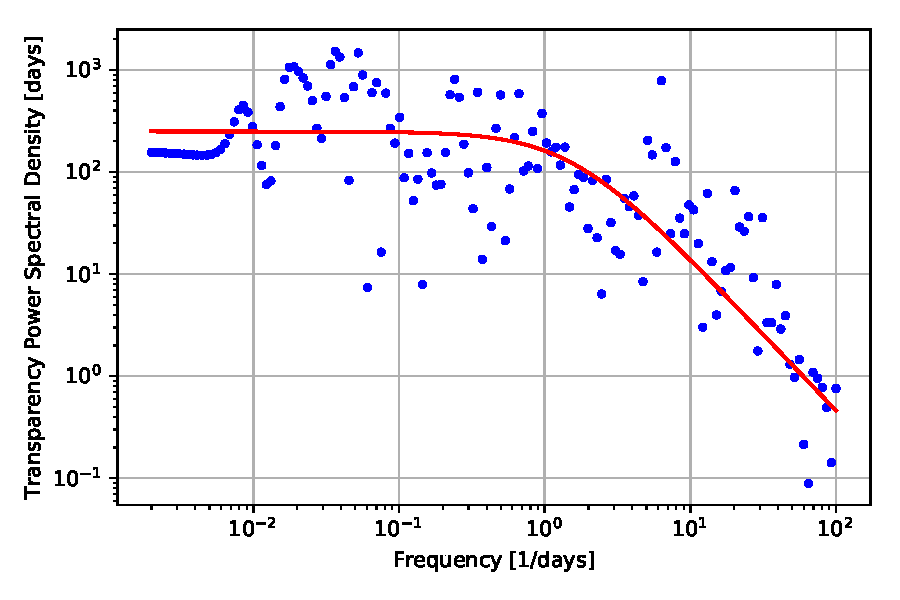
\includegraphics[width=0.48\linewidth]{transp-psd}
\caption{Power spectral density of whitened seeing (left) and corrected seeing (right) estimated using a Lomb-Scargle periodogram.  Smooth fits to piece-wise power laws are superimposed.}
\label{fig:transp-model}
\end{center}
\end{figure}

\begin{figure}[htb]
\begin{center}
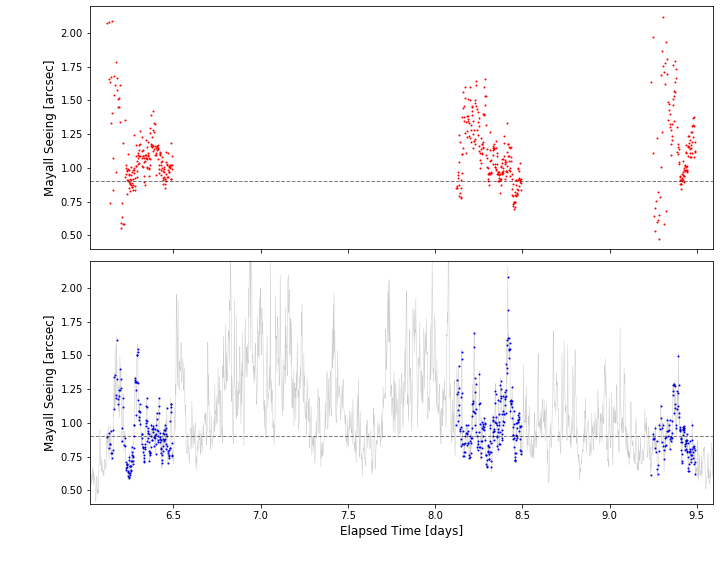
\includegraphics[width=6in]{seeing-sim}
\caption{Actual (upper) and simulated (lower) time series of atmospheric seeing. Dots show the times of actual MzLS observations. The gray line in the lower plot shows the continuous simulated time series passing through the simulated MzLS observations. The simulated data uses a median FWHM seeing of $0.923$ arcsec (indicated with dashed horizontal lines) to match the MzLS data.}
\label{fig:seeing-sim}
\end{center}
\end{figure}

\begin{figure}[htb]
\begin{center}
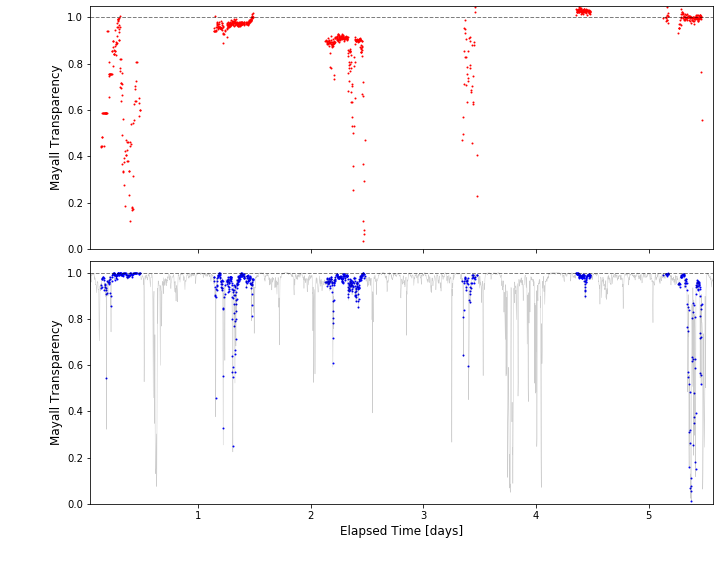
\includegraphics[width=6in]{transp-sim}
\caption{Actual (upper) and simulated (lower) time series of atmospheric transparency. Dots show the times of actual MzLS observations. The gray line in the lower plot shows the continuous simulated time series passing through the simulated MzLS observations. The data is corrected for dust accumulation on the primary mirror but includes Gaussian measurement errors.  The simulated values have the errors deconvolved, so represent true transparency and never exceed one.}
\label{fig:transp-sim}
\end{center}
\end{figure}

\subsection{Survey Planning Implications}

Atmospheric seeing and transparency over the course of the DESI survey are effectively random variables that add a stochastic component to exposure times.  For the purposes of survey planning, it is useful to summarize the impact of seeing and transparency variations with an overall exposure-time factor.  The relevant quantity is the increase $F_x$ in the nominal exposure time $T_0$ with nominal conditions $x_0$ required to achieve the same integrated signal to noise, i.e.
$$
\nu(F_x T_0) = \nu_0(T_0)
$$
where $\nu(T)$ is the integrated signal to noise,
$$
\nu(T) \equiv \int_0^T f(x(t))^{-1} dt
$$
and $f(x)$ models the instantaneous effect of parameter $x$ on signal to noise:
$$
\frac{d\nu}{dt}(x) = f(x)^{-1} \; .
$$
The parameter $x_0$ is the nominal value used to define the nominal total exposure time $T_0$ via
$$
\nu_0(T_0) = T_0 / f(x_0) \; .
$$

We can use the simulated time series describe above to numerically estimate $F_x$ as
$$
F_x = \left[ \frac{1}{N} \sum_{i=1}^N \frac{f(x_0)}{f(x_i)}\right]^{-1} \; ,
$$
where the $x_i$ are random samples at equally spaced times. To understand the scaling of $F_x$ with the statistical properties of $x$, it is also useful to approximate
\begin{align*}
\nu(T) &= \int_0^T f(x(t))^{-1}\, dt \\
&= \int_0^T (1/f)\left(
\mu_x + (x(t) - \mu_x)\right) \\
&\simeq \int_0^T \left[ (1/f)(\mu_x) + (1/f)'(\mu_x) (x - \mu_x)
+ \frac{1}{2} (1/f)''(\mu_x) (x - \mu_x)^2 \right]^{-1} \\
&= \frac{T}{f(\mu_x)}\left[1 + g(\mu_x) \sigma_x^2 \right] \; ,
\end{align*}
with
$$
g(x) \equiv \frac{f'(x)^2}{f(x)^2} - \frac{f''(x)}{2 f(x)} \; .
$$
This Taylor expansion approach leads to the estimate:
$$
\tilde{F}_x = \frac{f(\mu_x)}{f(x_0)} \left[1 +
g(\mu_x) \sigma_x^2 \right]^{-1} \; ,
$$
where $\mu_x$ ($\sigma_x$) are the mean (RMS) of the distribution of $x$. \tab{expfac} summarizes the results of both of these approaches for atmospheric seeing and transparency, assuming
$$
f(x) = 1/x
$$
for transparency, and
$$
f(x) = a + b x + c x^2 \quad , \quad (a,b,c) = (4.6, -1.55, 1.15)
$$
for seeing.  Note that the transparency exposure-time factor depends only on $\mu_x$ since $f(x)^{-1}$ is linear in $x$, leading to $g(\mu) = 0$ and $F_x = x_0 / \mu_x$.

\begin{table}[htb]
\begin{center}
\begin{tabular}{lcccccccc}
Condition & Nominal & Model & Median & $\mu_x$ & $\sigma_x$ & $g(\mu_x)$ & $\tilde{F}_x$ & $F_x$ \\
\hline
Seeing & $1.1$" & Old & $1.16$ & $1.28$ & $0.49$ & $-0.16$ & $1.09$ & $1.08$ \\
              & & New & $1.00$ & $1.06$ & $0.31$ & $-0.23$ & $1.01$ & $1.01$ \\
              & &     & $1.10$ & $1.17$ & $0.34$ & $-0.20$ & $1.04$ & $1.03$ \\
              & &     & $1.20$ & $1.27$ & $0.37$ & $-0.16$ & $1.07$ & $1.06$ \\
\hline
Transparency & $1.0$ & Old & $1.00$ & $0.93$ & $0.12$ & $0.00$ & $1.08$ & $1.08$ \\
             &       & New & $0.98$ & $0.94$ & $0.14$ & $0.00$ & $1.06$ & $1.06$ \\
\hline
\end{tabular}
\caption{Summary of simulated weather study to estimate the time-integrated exposure factors due to variable atmospheric seeing and transparency.  ``Old'' refers to the original simulation models implemented in {\tt desimodel.seeing} and {\tt surveysim.weather}.  ``New'' refers to the new model based on MzLS data described here. The last two columns provide the Taylor-series estimate $\tilde{F}_x$ and the simulated numerical estimate $F_x$ described in the text.}
\label{tab:expfac}
\end{center}
\end{table}

The overall conclusion from these studies is that the new models derived from MzLS observations predict that actual atmospheric conditions will increase the exposure time by about 9\% relative to nominal conditions, which is lower than the 17\% predicted by the old models.

\def\pasp{PASP} %Publications of the Astronomical Society of the Pacific

\bibliographystyle{unsrt}
\bibliography{weather}

\end{document}
